\documentclass[11pt]{article}
\usepackage[toc,page]{appendix}
\usepackage{amsmath, amssymb}
\usepackage[utf8]{inputenc}
\usepackage[T1]{fontenc}
\usepackage[style=apa,backend=biber]{biblatex}
%\usepackage{biblatex}
\addbibresource{references.bib}
\usepackage{graphicx}
\usepackage{tikz}
\usetikzlibrary{automata,positioning,shapes.geometric, arrows.meta, fit, backgrounds, calc, chains}
\graphicspath{./images/Easy_Pictures/SMR_MULT_Repackaging}%\usepackage{kpfonts}
\usepackage{float}
\usepackage[margin=1in]{geometry}
\usepackage{cancel}
\usepackage{epsfig}
\usepackage{tikz-3dplot}
\usepackage{darkmode}
\usepackage{dirtytalk}
\usepackage{longtable,booktabs,array}
\usepackage{calc} % for calculating minipage widths
\usepackage[utf8]{inputenc}
\usepackage[T1]{fontenc}
\usepackage{xcolor}
\usepackage{listings}


\usepackage{etoolbox}
\usepackage{hyperref}
\hypersetup{
    colorlinks=true,
    linkcolor=blue,
    filecolor=magenta,      
    urlcolor=cyan,
    pdftitle={Hermeneutic Calculator},
    citecolor=blue,
    }


\urlstyle{same}

\lstdefinestyle{htmlStyle}{
    language=HTML,
    basicstyle=\ttfamily\small,
    keywordstyle=\color{blue}\bfseries,
    commentstyle=\color{gray}\itshape,
    stringstyle=\color{red},
    breaklines=true,
    frame=single,
    numbers=left,
    numberstyle=\tiny\color{gray},
    columns=fullflexible,
}
\lstdefinelanguage{HTML}{
  keywords={<!DOCTYPE, html, head, title, body, h1, h2, h3, p, div, span, a, img, ul, li, table, tr, td, th, style, link, script},
  sensitive=true,
  comment=[l]{//},
  morecomment=[s]{/*}{*/},
  morestring=[b]',
  morestring=[b]"
}
\lstset{style=htmlstyle, language=html}
% Updated to explicitly pass the language option
%\lstinputlisting[style=htmlstyle, language=html]{./html/example.html}
%\usepackage{tocloft}

% Optional: define some custom colors
\definecolor{sliceRed}{RGB}{225,224,91} % matching "varyellow" from your code
\definecolor{linkYellow}{RGB}{255,215,0}  % a golden yellow
\tdplotsetmaincoords{70}{110}

\title{Addition Strategies: Counting On By Bases and then Ones (COBO)}
\author{Compiled by: Theodore M. Savich}


\begin{document}
\maketitle
\subsection*{Transcript}
Video from \textcite{Carpenter1999}. Strategy descriptions and examples adapted from \textcite{HackenbergCourseNotes}. 
\begin{itemize}
\item \textbf{Teacher:} Max  has  46  comic  books. For  his  birthday,  his  father  gives him  37  more  comic  books. How  many  comic  books  does  Max  have  now? 

\item \textbf{Lauren:} Forty-six  \ldots 
\item \textbf{Teacher:} He  gets  37  more  for  his  birthday. 
\item  \textbf{Lauren:} Ok. 46,  56, 66,  76,  77, 78,  79,  80,  81, 82,  83. It's  83. 
\item \textbf{Teacher:} Good  work.
\end{itemize}

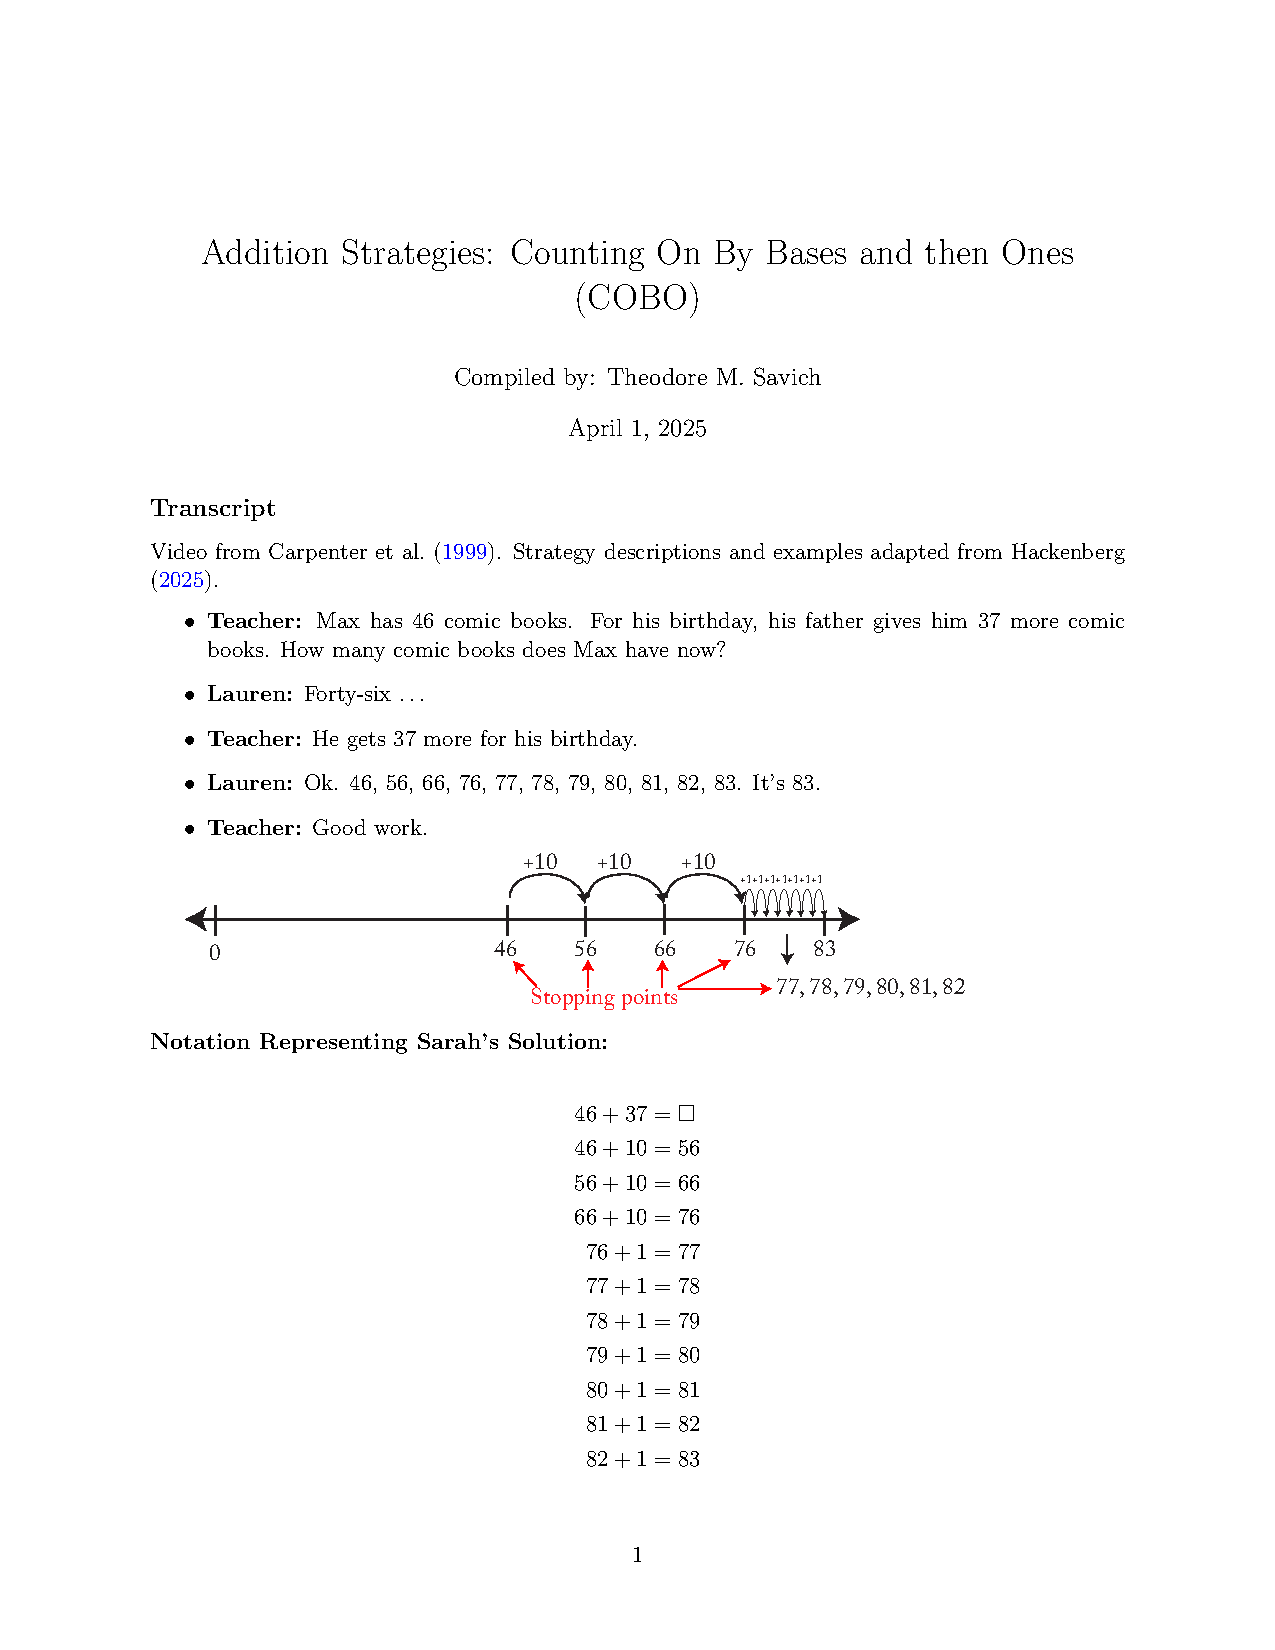
\includegraphics[width=.8\textwidth]{images/Easy_Pictures/SAR_ADD_COBO/PDF/SAR_ADD_COBO.pdf}

\noindent \textbf{Notation Representing Sarah's Solution:}

\begin{align*}
46 + 37 &= \Box \\
46+10 &= 56\\
56+10 &= 66\\
66+10 &= 76\\
76+1 &= 77\\
77+1 &= 78\\
78+1 &= 79\\
79+1 &= 80\\
80+1 &= 81\\
81+1 &= 82\\
82+1 &= 83\\
\end{align*}

\subsubsection*{Description of Strategy:}

 \textbf{Objective:} Description of Counting On by Bases and Then Ones (COBO)
 Begin with one of the numbers. Break the other number into its base units and its ones. Then, “count on” by adding each base unit one at a time, followed by each individual one.
 
 Why are number lines useful for demonstrating this strategy?
 COBO is essentially a jump strategy—you start at one number and make “jumps” equal to the other number’s base units, then add in the remaining ones. Number lines are ideal because they visually display jumps of varying lengths and directions. They serve as a picture of the process: a jump representing a full base is clearly larger (by a factor of the base) than a jump of a single unit.
 
 Good number line illustrations should:
\begin{itemize}
 \item Clearly represent the relative sizes of the jumps—each base jump should be exactly as many times larger than a single-unit jump as the base indicates, with all base jumps the same size and all one-unit jumps identical.
 \item Indicate the position of 0, or mark a break if that portion of the line isn’t drawn to scale.
 \item Use arrows to indicate direction—when adding, the jumps go to the right (or upward); when subtracting, they go to the left (or downward).
 \item Mark all landing points clearly—the numbers you would speak aloud when counting on by bases and then ones, just as Lauren demonstrated.
\end{itemize}

\subsection*{Counting On by Bases and Then Ones (COBO)}

\subsubsection*{Description of Strategy}
\begin{itemize}
    \item \textbf{Objective:} Start with one addend, add bases from the other addend one by one, then add ones one by one.
    \item \textbf{Example:} \(46 + 37\)
    \begin{itemize}
        \item Start at \(46\).
        \item Add tens one by one: \(46 \rightarrow 56 \rightarrow 66 \rightarrow 76\).
        \item Add ones one by one: \(76 \rightarrow 77 \rightarrow \ldots \rightarrow 83\).
    \end{itemize}
\end{itemize}

\subsubsection*{Automaton Type}
\textbf{Finite State Automaton (FSA) with Counters}:  
Counters are used to manage the repeated addition:
\begin{itemize}
    \item \textbf{BaseCounter:} Number of base units (e.g., tens) to add.
    \item \textbf{OneCounter:} Number of ones to add.
    \item \textbf{Sum:} The running total.
\end{itemize}

\subsubsection*{Formal Description of the Automaton}

We define the automaton as the tuple
\[
M = (Q,\,\Sigma,\,\delta,\,q_{0/accept},\,F,\,C)
\]
where:
\begin{itemize}
    \item \(Q = \{q_{0/accept},\, q_1,\, q_2,\, q_3\}\) is the finite set of states. Here, the start state \(q_{0/accept}\) is also the accept state.
    \item \(\Sigma = \{0,1,2,3,4,5,6,7,8,9,+\}\) is the input alphabet (suitable for representing the addends).
    \item \(F = \{q_{0/accept}\}\) is the set of accepting states.
    \item \(C = \{\text{BaseCounter},\; \text{OneCounter},\; \text{Sum}\}\) is the set of counters.
    \item \(\delta\) is the transition function defined by:
    \begin{enumerate}
        \item \(\delta(q_{0/accept},\, \text{``}A,B\text{''}) = (q_1,\; \text{update: } \text{Sum} \gets A,\; \text{BaseCounter} \gets \lfloor B/10 \rfloor,\; \text{OneCounter} \gets B \bmod 10 )\) \\
              (Read inputs \(A\) and \(B\); initialize the Sum to \(A\) and set the counters based on \(B\).)
        \item \(\delta(q_1,\, \varepsilon) = (q_2,\; \text{if BaseCounter} > 0)\) \\
              (If there are base units to add, proceed to add them.)
        \item \(\delta(q_2,\, \varepsilon) = (q_2,\; \text{update: } \text{Sum} \gets \text{Sum} + \text{baseUnit},\; \text{BaseCounter} \gets \text{BaseCounter} - 1)\) \\
              (In state \(q_2\), repeatedly add one base unit (e.g., 10) to Sum while decrementing BaseCounter.)
        \item \(\delta(q_2,\, \varepsilon) = (q_3,\; \text{if BaseCounter} = 0)\) \\
              (When no more base units remain, switch to adding ones.)
        \item \(\delta(q_3,\, \varepsilon) = (q_3,\; \text{update: } \text{Sum} \gets \text{Sum} + 1,\; \text{OneCounter} \gets \text{OneCounter} - 1)\) \\
              (In state \(q_3\), repeatedly add 1 to Sum while decrementing OneCounter.)
        \item \(\delta(q_3,\, \varepsilon) = (q_{0/accept},\; \text{if OneCounter} = 0)\) \\
              (When OneCounter reaches 0, output the final Sum and return to the closed start/accept state.)
    \end{enumerate}
\end{itemize}

\subsubsection*{Automaton Diagram for COBO}

The following diagram arranges the four states on a circle with \(q_{0/accept}\) serving as both the start and accept state.

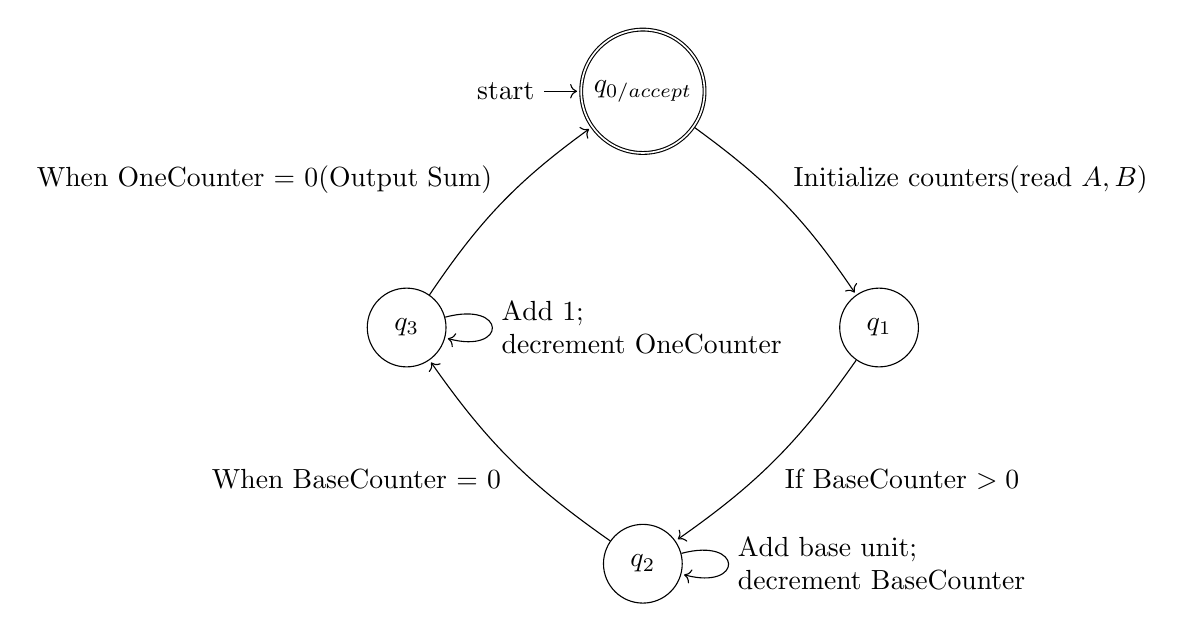
\begin{tikzpicture}[
    shorten >=1pt,
    on grid,
    auto,
    every state/.style={minimum size=1cm}
]
    % Define radius and starting angle
    \def\radius{3cm}
    \def\startangle{90}
    \def\incangle{360/4} % Four states equally spaced

    % Nodes arranged on a circle
    \node[state, initial, accepting] (q0) at (\startangle:\radius) {$q_{0/accept}$};
    \node[state] (q1) at ({\startangle-\incangle}:\radius) {$q_1$};
    \node[state] (q2) at ({\startangle-2*\incangle}:\radius) {$q_2$};
    \node[state] (q3) at ({\startangle-3*\incangle}:\radius) {$q_3$};

    % Transitions between states
    \path[->]
        (q0) edge[bend left=10] node {Initialize counters \\ (read \(A,B\))} (q1)
        (q1) edge[bend left=10] node[align=left] {If BaseCounter \(>0\)} (q2)
        (q2) edge[loop right] node[align=left] {Add base unit; \\ decrement BaseCounter} (q2)
        (q2) edge[bend left=10] node {When BaseCounter = 0} (q3)
        (q3) edge[loop right] node[right, align=left] {Add 1; \\ decrement OneCounter} (q3)
        (q3) edge[bend left=10] node {When OneCounter = 0 \\ (Output Sum)} (q0);
\end{tikzpicture}

\clearpage
\subsubsection*{HTML Implementation}
\lstinputlisting[style=htmlStyle, language=html]{./new_html/SAR_ADD_COBO.html}

\printbibliography
\end{document}